\section{Histograms}
\subsection{Tennis.png RGB Histograms}
The Tennis.png file was loaded using a similar method as before. Once the image was loaded, I separated the channels and passed each component to the histogram function in MATLAB which calculated the bins and produced the histogram. This is shown in Figure \ref{fig:TennisRGBHistogram}

\begin{figure}[!h]
    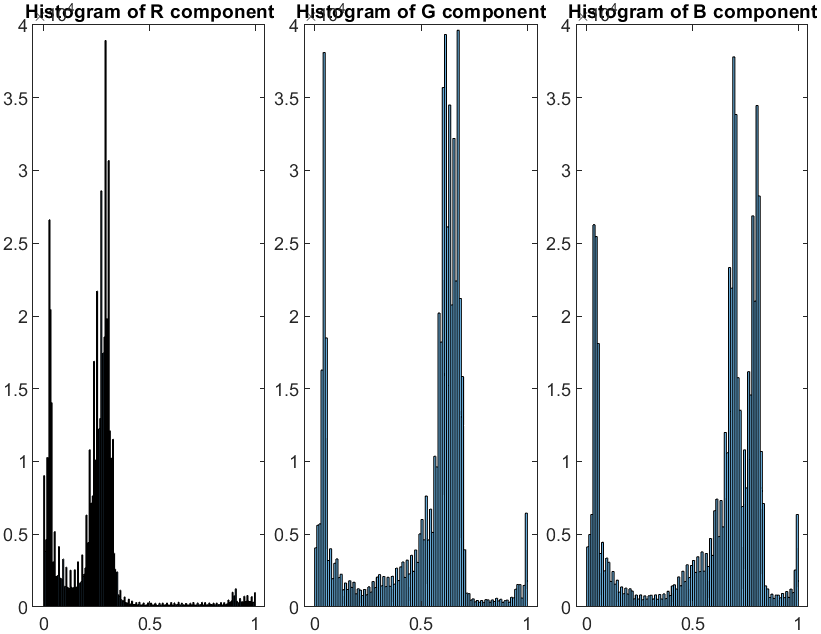
\includegraphics[width=1\textwidth]{TennisHistogramsRGB.png}
    \centering
    \caption{Histograms of the R, G and B components of Tennis.png}
    \label{fig:TennisRGBHistogram}
\end{figure}

\subsection{Conversion to YCbCr}
Converting to the YCbCr space was as easy as calling the rgb2ycbcr function in MATLAB. The output of the function is shown in Figure \ref{fig:TennisYCbCr}.

\begin{figure}[!h]
    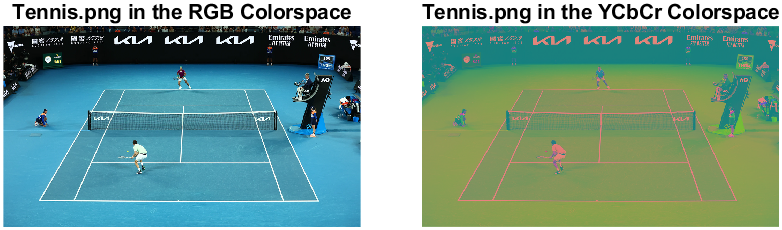
\includegraphics[width=1\textwidth]{TennisRGBvsYCbCr.png}
    \centering
    \caption{A comparison of Tennis.png in the RBG and YCbCr Color Space}
    \label{fig:TennisYCbCr}
\end{figure}

\subsection{Tennis.png YCbCr Histograms}
Shown below are the histograms after the image was converted to the YCbCr Color space.

\begin{figure}[!h]
    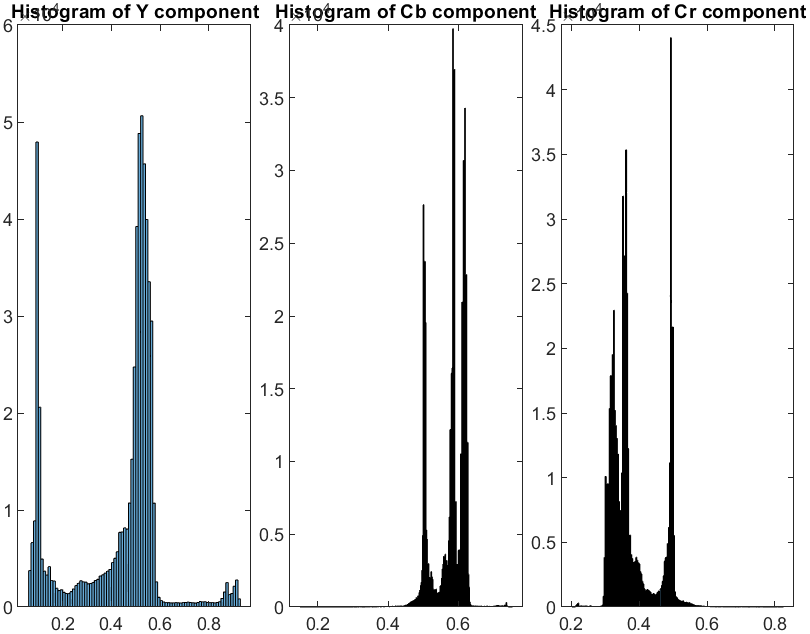
\includegraphics[width=1\textwidth]{TennisHistogramsYCbCr.png}
    \centering
    \caption{Histograms of the Y, Cb and Cr components of Tennis.png}
    \label{fig:TennisYCbCrHistogram}
\end{figure}

\subsection{Interpreting Histograms}
\label{sec:SubSecInterpretingHistograms}
Histograms allow us to see the distribution of the color components in our image. These are extensively used in color-grading applications for movies and TV shows. It allows graphics artists to hone in on the exact color profile that they envision. However, the information provided by the histograms can also be used to segment large objects in an image. The idea behind this is that large objects that are relatively homogeneous in color, will appear as spikes on the histograms. This can be seen in the YCbCr histograms in Figure \ref{fig:TennisYCbCrHistogram}. Large spikes can be seen on the Y component around 0.57, on the Cb component around 0.56, and on the Cr component around 0.48. We can then use these values as a threshold and create a mask that will only select the pixels that are above this threshold.